\documentclass[usenames,dvipsnames,aspectratio=169]{beamer}
\usepackage{../common/prg}

\title[5. előadás]{Programozás}
\subtitle{(GKxB\_INTM114)}

\begin{document}

%1
\begin{frame}[plain]
  \titlepage
  \logoalul
\end{frame}

%2
\section{Függvények}
\subsection{Általános jellemzők}
\begin{frame}
  Mi az a függvény (function)?
  \begin{itemize}
    \item[] Programkód egy konkrét, azonosítható, paraméterezhető, újrahasznosítható blokkja
  \end{itemize}
  \vfill
  Miért használunk függvényeket?
  \begin{itemize}
    \item Hosszú forrásszöveg áttekinthető, kisebb részekre tördelése (modularitás)
    \item Többszöri felhasználás lehetősége
    \begin{itemize}
      \item egy programon belül, kódismétlés nélkül
      \item több programban, gyakran használt részeket nem kell újra megírni (ld. \texttt{sqrt}, \texttt{pow})
    \end{itemize}
  \end{itemize}
\end{frame}

%3
\subsection{Függvény definíciója}
\begin{frame}
  Függvény definíció (definition)
  \begin{itemize}
    \item Teljes formai információ a függvényről
    \begin{itemize}
      \item visszatérési érték típusa (return type)
      \item azonosító (name)
      \item \emph{formális} paraméterek (parameters)
      \item függvénytest (body, ld. \texttt{main})
    \end{itemize}
    \item Pontosan egy létezhet belőle
    \item Forrásfájlokban vagy előfordított könyvtárakban tárolják
  \end{itemize}
  \begin{exampleblock}{\textattachfile{abszolut3.cpp}{abszolut3.cpp} Abszolútérték számítás függvénnyel}
    \small
    \vspace{-.2cm}
    \lstinputlisting[style=cpp,linerange={4-6},numbers=left,firstnumber=4]{abszolut3.cpp}
    \vspace{-.2cm}
  \end{exampleblock}
\end{frame}

%4
\subsection{Függvény hívása}
\begin{frame}
  \small
  Függvényhívás (call, invoke)
  \begin{compactitem}
    \item A függvénynek a híváskor ismertnek kell lennie
    \item Vezérlés + \emph{aktuális} paraméterek átadása
    \item \emph{Érték szerinti} paraméterátadás (pass by value)
    \item Vezérlés visszaadása + visszatérési érték szolgáltatása: \texttt{return}
  \end{compactitem}
  \footnotesize
  \begin{exampleblock}{\textattachfile{abszolut3.cpp}{abszolut3.cpp}}
    \footnotesize
    \vspace{-.2cm}
    \lstinputlisting[style=cpp,linerange={8-17},numbers=left,firstnumber=8]{abszolut3.cpp}
    \vspace{-.2cm}
  \end{exampleblock}
\end{frame}

%5
\subsection{Függvény visszatérési értéke, formális paraméterei}
\begin{frame}
  Visszatérési érték
  \begin{itemize}
    \item Vt. típusa \kiemel{nem lehet tömb}
    \item \texttt{return} utáni kifejezés: \hiv{\href{https://learn.microsoft.com/en-us/cpp/c-language/assignment-conversions?view=msvc-170}{\emph{hozzárendelési}}} konverzió szükséges lehet
    \item \texttt{void} típus: valaminek a hiányát jelzi (\hiv{\href{https://wiki.freepascal.org/Procedure}{,,eljárás''}})
  \end{itemize}
  \vfill
  Formális paraméterlista
  \begin{itemize}
    \item Nincsenek paraméterek: \texttt{int main() \{...\}}
    \item Egy paraméter: \texttt{double abszolut(double szam) \{...\}}
    \item Két paraméter: \texttt{double hatvany(double alap, double kitevo) \{...\}}
    \item Aktuális paraméterek (arguments) $\to$ hozzárendelési konverzió $\to$ formális paraméterek
    \item Tömb átadása speciális eset
  \end{itemize}
\end{frame}

%6
\subsection{Függvény teste}
\begin{frame}
  A függvény teste tartalmazhat mindent, ami a \texttt{main}-ben is megengedett volt, azaz
  \begin{compactitem}
    \small
    \item Változók deklarációit
    \item A blokkon kívül deklarált tételekre történő hivatkozásokat
    \item Tevékenységet meghatározó utasításokat
  \end{compactitem}
  \vfill
  Visszatérés a függvényből
  \begin{compactitem}
    \small
    \item a függvény végén
    \item \texttt{return} utasítással (a fv. tartalmazhat több \texttt{return}-t is)
  \end{compactitem}
  \vfill
  \begin{exampleblock}{\textattachfile{keres.cpp}{keres.cpp} Karakter első előfordulásának keresése \texttt{string}-ben}
    \footnotesize
    \vspace{-.2cm}
    \lstinputlisting[style=cpp,linerange={4-9},numbers=left,firstnumber=4]{keres.cpp}
    \vspace{-.2cm}
  \end{exampleblock}
\end{frame}

%7
\begin{frame}
  Függvények definíciói \kiemel{nem ágyazhatóak egymásba}!
  \begin{exampleblock}{\textattachfile{beagyazas.cpp}{beagyazas.cpp}}
    \small
    \vspace{-.2cm}
    \lstinputlisting[style=cpp,numbers=left]{beagyazas.cpp}
    \vspace{-.2cm}
  \end{exampleblock}
  \begin{block}{Fordítási hiba}
    \scriptsize
beagyazas.cpp: In function 'int main()':\\
beagyazas.cpp:2:32: error: a \kiemel{function-definition is not allowed here} before '\{' token\\
  double abszolut(double szam) \{\\
  \end{block}
\end{frame}

%8
\subsection{Hozzárendelési konverzió}
\begin{frame}
  Implicit típuskonverzióra szükség lehet amikor egy változóhoz új értéket rendelnek, pl. fv. visszatérési értékének kialakításakor.
  \vfill
  \begin{exampleblock}{\textattachfile{keres.cpp}{keres.cpp} \texttt{size\_t} $\to$ \texttt{signed int}}
    \lstinputlisting[style=cpp,linerange={4-9},numbers=left,firstnumber=4]{keres.cpp}
  \end{exampleblock}
\end{frame}

%9
\begin{frame}
  Hasonlóan, pl. függvény aktuális paraméterének konverziójánál.
  \vfill
  \begin{exampleblock}{\textattachfile{abszolut3.cpp}{abszolut3.cpp} \texttt{int} $\to$ \texttt{double}}
    \lstinputlisting[style=cpp,linerange={4-6},numbers=left,firstnumber=4]{abszolut3.cpp}
    \lstinputlisting[style=cpp,linerange={12-12},numbers=left,firstnumber=12]{abszolut3.cpp}
  \end{exampleblock}
\end{frame}

%10
\begin{frame}
  Az \hiv{\href{http://en.cppreference.com/w/c/language/conversion}{implicit típuskonverzió}} részletei\\
  Néhány példa:
  \begin{table}
    \begin{tabular}{lll}
    Miről?   & Mire?    & Kimenetel                 \\ \hline
    signed+  & unsigned & \kiemelZ{\checkmark}      \\
    signed$-$ & unsigned & \kiemel{előjel funkcióvesztése} \\
    long int & int      & értékvesztés veszélye     \\
    int      & double   & értékvesztés veszélye \\
    float    & double   & \kiemelZ{\checkmark}      \\
    double   & float    & pontosságvesztés veszélye \\
    double   & int      & \kiemel{törtrész levágás} \\
    \end{tabular}
  \end{table}
\end{frame}

%11
\subsection{Mintapélda függvények használatára}
\begin{frame}
  Minta alkalmazás megvalósítandó szolgáltatásai (függvények):
  \vfill
  \begin{description}[mm]
    \item[Kombináció] Adott $n$ különböző elem. Ha $n$ elem közül $k (0 < k \leq n)$ elemet úgy választunk ki, 
hogy mindegyik csak egyszer kerül sorra, és a kiválasztás sorrendje nem számít, akkor az $n$ elem egy $k$-ad osztályú ismétlés 
nélküli kombinációját kapjuk. Jele: $C_n^k$\\
    \vfill
    $C_n^k = \frac{n!}{(n-k)!k!} = {n \choose k}$\\
    \vfill
    Példa: hányféleképpen tudunk \emph{három} gyümölcs (mondjuk \kiemelZ{alma}, \kiemelN{körte}, \kiemel{barack}) közül 
\emph{kettőt} kiválasztani?
    \begin{enumerate}
      \item \kiemelZ{alma}, \kiemelN{körte}
      \item \kiemelZ{alma}, \kiemel{barack}
      \item \kiemelN{körte}, \kiemel{barack}
    \end{enumerate}
  \end{description}
\end{frame}

%12
\begin{frame}
  \begin{description}[mm]
    \item[Faktoriális] Egy $n$ nemnegatív egész szám faktoriálisa az $n$-nél kisebb vagy egyenlő pozitív egész számok 
szorzata. Jele: $n!$\\
    $n! = \prod_{k=1}^{n}k$ minden $n \geq 0$ számra.\\
    Megállapodás szerint $0! = 1$\\
    $n$ elemet $n!$ sorrendbe lehet állítani (permutációk)\\
    Példa: hányféleképpen tudunk \emph{három} gyümölcsöt (mondjuk \kiemelZ{alma}, \kiemelN{körte}, \kiemel{barack}) sorba 
állítani?
    \begin{enumerate}
      \item \kiemelZ{alma}, \kiemelN{körte}, \kiemel{barack}
      \item \kiemelZ{alma}, \kiemel{barack}, \kiemelN{körte}
      \item \kiemelN{körte}, \kiemelZ{alma}, \kiemel{barack}
      \item \kiemelN{körte}, \kiemel{barack}, \kiemelZ{alma}
      \item \kiemel{barack}, \kiemelZ{alma}, \kiemelN{körte}
      \item \kiemel{barack}, \kiemelN{körte}, \kiemelZ{alma}
    \end{enumerate}
  \end{description}
\end{frame}

%13
\begin{frame}
  \begin{description}[mm]
    \item[Beolvasás] Beolvasandó $n$ és $k$ értéke
    \item[Főprogram] Adatok beolvasása, ${n \choose k}$ megjelenítése
  \end{description}
  \vfill
  \begin{center}
    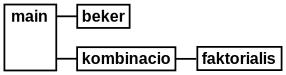
\includegraphics{nk1.pdf}
  \end{center}
\end{frame}

%14
\begin{frame}
  \begin{center}
    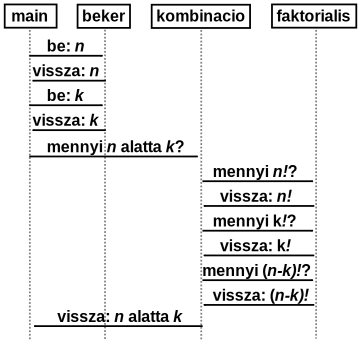
\includegraphics[scale=0.75]{nk2.pdf}
  \end{center}
\end{frame}

%15
\begin{frame}
  \begin{exampleblock}{\textattachfile{nk1.cpp}{nk1.cpp}}
    \meret{9}
    \vspace{-.2cm}
    \lstinputlisting[style=cpp,linerange={1-15},numbers=left]{nk1.cpp}
    \vspace{-.2cm}
  \end{exampleblock}
\end{frame}

%16
\begin{frame}
  \begin{exampleblock}{\textattachfile{nk1.cpp}{nk1.cpp}}
    \meret{7}
    \vspace{-.2cm}
    \lstinputlisting[style=cpp,firstline=17,numbers=left,firstnumber=17]{nk1.cpp}
    \vspace{-.2cm}
  \end{exampleblock}
\end{frame}

%17
\subsection{Függvény felültöltése}
\begin{frame}
  \small
  A függvényt a neve és paramétereinek száma, típusa együttesen azonosítja. A felültöltött (overload) változatok közül  
  híváskor az aktuális paraméterek alapján \hiv{\href{https://en.cppreference.com/w/cpp/language/overload\_resolution}{választ}}.
  \begin{columns}[T]
    \column{0.47\textwidth}
      \begin{exampleblock}{\textattachfile{nk2.cpp}{nk2.cpp} -- \texttt{beker()}}
        \scriptsize
        \lstinputlisting[style=cpp,linerange={4-15},numbers=left,firstnumber=4]{nk2.cpp}
      \end{exampleblock}
    \column{0.47\textwidth}
      \begin{exampleblock}{\textattachfile{nk2.cpp}{nk2.cpp} -- \texttt{beker(int)}}
        \scriptsize
        \lstinputlisting[style=cpp,linerange={17-28},numbers=right,firstnumber=17]{nk2.cpp}
      \end{exampleblock}
  \end{columns}
\end{frame}

%18
\subsection{Alapértelmezett függvényparaméterek}
\begin{frame}
  Alapértelmezett függvényparaméterek: 
  \begin{itemize}
    \small
    \item Egy paraméternek alapértelmezett értéket adunk $\to$ tőle jobbra lévőknek is adni kell!
    \item Híváskor nem adunk át értéket egy alapértelmezett paraméternek $\to$ ettől jobbra lévők se kaphatnak!
  \end{itemize}
  \begin{exampleblock}{\textattachfile{nk3.cpp}{nk3.cpp}}
    \scriptsize
    \vspace{-.2cm}
    \lstinputlisting[style=cpp,linerange={5-15},numbers=left,firstnumber=5]{nk3.cpp}
    \vspace{-.2cm}
  \end{exampleblock}
\end{frame}

%19
\section{Fogalmak}
\subsection{Élettartam}
\begin{frame}
  \kiemel{Élettartam} (lifetime, duration): az a \emph{periódus a futásidő alatt}, amíg a változó/függvény létezik, memóriát 
  foglal. \hiv{\href{https://en.cppreference.com/w/cpp/language/lifetime}{Részletek}}. Típusai:
  \begin{itemize}
    \item Statikus
    \begin{itemize}
      \item Futás kezdetétől végéig foglal memóriát
      \item Összes függvény, és \emph{globális} (függvényeken kívül deklarált) változó ilyen
      \item Globális változók implicit inicializálása: minden bit zérus értékű
      \item Lehetőleg \kiemel{kerülni kell a globális változók használatát}
      \begin{itemize}
        \item[$+$] Paraméter-átadás költsége megtakarítható
        \item[$-$] Nehézkes újrahasznosíthatóság, rugalmatlan, környezetfüggő kód, névütközések veszélye, \dots
      \end{itemize}
    \end{itemize}
  \end{itemize}
\end{frame}

%21
\begin{frame}
  \begin{columns}[T]
    \column{0.46\textwidth}
      \begin{itemize}
      \small
      \item Lokális
      \begin{itemize}
        \item blokkba belépéstől, vagy a definíció sorát elérve, a blokk elhagyásáig rendelnek memóriát hozzájuk
        \item függvényparaméterek, vezérlési szerkezetek blokkjai is ilyenek
        \item csak explicit inicializáció történhet
      \end{itemize}
    \end{itemize}
    \column{0.5\textwidth}
      \begin{exampleblock}{\textattachfile{nk1.cpp}{nk1.cpp}}
        \tiny
        \lstinputlisting[style=cpp,linerange={17-24},numbers=right,firstnumber=17]{nk1.cpp}
      \end{exampleblock}
  \end{columns}
  \vfill
  \scriptsize
  Élettartamok:
  \begin{description}[]
    \item[faktorialis] program teljes futásideje alatt létezik
    \item[$n$] 3 fv. hívás miatt 3x létrejön a fv. hívásakor/megszűnik visszatéréskor (17-23. sor)
    \item[$f$] létrejöhet pl. a függvény hívását követően és megszűnik amikor a végrehajtás a 23. sorhoz ér
    \item[$i$] a 20. sor elérése pillanatában jön létre, és a ciklusból kilépéskor felszabadul
  \end{description}
\end{frame}

%21
\subsection{Hatáskör}
\begin{frame}
  \kiemel{Hatáskör} (érvényességi tartomány, hatókör, scope): meghatározza, hogy valamit a program \emph{mely részén} 
  lehet elérni. \hiv{\href{https://en.cppreference.com/w/cpp/language/scope}{Részletek}}. Deklarációtól és annak helyétől függően:
  \begin{itemize}
    \item Blokk (lokális, belső)
    \begin{itemize}
      \item Deklarációtól a tartalmazó blokk végéig, beleértve a beágyazott blokkokat is
      \item A beágyazott blokkban deklarált azonosító ideiglenesen elrejtheti 
      a befoglaló blokkban lévő azonosítót $\to$ \kiemel{rossz programozói gyakorlat, kerülendő!}
      \item Pl. függvény formális paraméterei, lokális változói
    \end{itemize}
    \item Fájl (globális, külső)
    \begin{itemize}
      \item minden függvény testén kívül deklarált azonosítók; deklarációs ponttól a fájl végéig
      \item Pl. függvények, globális változók
    \end{itemize}
  \end{itemize}
\end{frame}

%22
\section{Rekurzív függvények}
\subsection{Rekurzív faktoriális számítás}
\begin{frame}
  \kiemel{Rekurzív} függvényhívás
  \begin{itemize}
    \item Minden fv. hívhatja magát közvetlenül vagy közvetve (ön- és kölcsönös rekurzió)
    \item Minden hívásnál új területet foglalnak a formális paramétereknek, lokális változóknak
    \item A globális változók mindig ugyanazon a területen maradnak!
    \item El kell kerülni a végtelen mélységű rekurziót!
  \end{itemize}
  \begin{exampleblock}{\textattachfile{nk4.cpp}{nk4.cpp}}
    \lstinputlisting[style=cpp,linerange={17-20},numbers=left,firstnumber=17]{nk4.cpp}
  \end{exampleblock}
\end{frame}

%23
\subsection{Rekurzív hatványozás}
\begin{frame}
  \scriptsize
  \begin{exampleblock}{\textattachfile{hatvany1.cpp}{hatvany1.cpp} Hatványozás szorzásokra visszavezetve}
    \scriptsize
    \vspace{-.2cm}
    \lstinputlisting[style=cpp,linerange={4-9},numbers=left,firstnumber=4]{hatvany1.cpp}
    \vspace{-.2cm}
  \end{exampleblock}
  \begin{exampleblock}{\textattachfile{hatvany2.cpp}{hatvany2.cpp} Rekurzív hatványozás, pl. $-3^5 = {-3^2}^2 \times -3^1 = 
-243$}
    \scriptsize
    \vspace{-.2cm}
    \lstinputlisting[style=cpp,linerange={4-11},numbers=left,firstnumber=4]{hatvany2.cpp}
    \vspace{-.2cm}
  \end{exampleblock}
\end{frame}

%24
\subsection{Fibonacci-sorozat}
\begin{frame}
  \hiv{\href{https://hu.wikipedia.org/wiki/Fibonacci-sz\%C3\%A1mok}{Fibonacci-sorozat}}: másodrendben rekurzív sorozat. Képzeletbeli nyúlcsalád növekedése: hány pár nyúl lesz $n$ hónap múlva, ha
  \begin{itemize}
    \item az első hónapban csak egyetlen újszülött nyúl-pár van,
    \item az újszülött nyúl-párok két hónap alatt válnak termékennyé,
    \item minden termékeny nyúl-pár minden hónapban egy újabb párt szül,
    \item és a nyulak örökké élnek.
  \end{itemize}
  \vfill
  $F_n = \left\{ \begin{array}{ll}
    0, & \textrm{ha $n=0$}\\
    1, & \textrm{ha $n=1$}\\
    F_{n-1} + F_{n-2} & \textrm{ha $n>1$}
  \end{array} \right.$
\end{frame}

%25
\begin{frame}
  \scriptsize
  \begin{exampleblock}{\textattachfile{fibonacci1.cpp}{fibonacci1.cpp} Iteratív változat}
    \scriptsize
    \vspace{-.2cm}
    \lstinputlisting[style=cpp,firstline=4,lastline=13,numbers=left,firstnumber=4]{fibonacci1.cpp}
    \vspace{-.2cm}
  \end{exampleblock}
  \begin{exampleblock}{\textattachfile{fibonacci2.cpp}{fibonacci2.cpp} Rekurzív változat}
    \scriptsize
    \vspace{-.2cm}
    \lstinputlisting[style=cpp,firstline=4,lastline=7,numbers=left,firstnumber=4]{fibonacci2.cpp}
    \vspace{-.2cm}
  \end{exampleblock}
\end{frame}

\end{document}